\documentclass[]{beamer}

\usepackage[utf8]{inputenc}
\usepackage[danish]{babel}
\usepackage[T1]{fontenc}
\usepackage{graphicx}
\usepackage{amsmath}
\usepackage{hyperref}
\usepackage{enumerate}
\usepackage{url}

\renewcommand{\emptyset}{\varnothing}
\newcommand{\ignore}[1]{}
\newcommand{\f}[1]{\textcolor{red}{#1}}

%\let\originaltextperiodcentered\textperiodcentered
\renewcommand{\textperiodcentered}{\ensuremath{\cdot}}
\newcommand{\explain}[2]{\underset{\mathclap{#2}}{\underbrace{#1}}}
\newcommand{\putat}[3]{\begin{picture}(0,0)(0,0)\put(#1,#2){#3}\end{picture}}

\def\imagetop#1{\vtop{\null\hbox{#1}}}

\newenvironment<>{varblock}[2][\textwidth]{%
  \setlength{\textwidth}{#1}
  \begin{actionenv}#3%
    \def\insertblocktitle{#2}%
    \par%
    \usebeamertemplate{block begin}}
  {\par%
    \usebeamertemplate{block end}%
  \end{actionenv}}

\setbeamertemplate{navigation symbols}{} 
\setbeamertemplate{items}[circle]
\useoutertheme{infolines} 
\setbeamercovered{transparent=40} 

\title{2. Seminar EVU RegAut}
\author{Sigurd Meldgaard}
\date{10. spetember 2010}

\AtBeginSection[]
{
   \begin{frame}
       \frametitle{Plan}
       \tableofcontents[currentsection]
   \end{frame}
}

\begin{document}
\maketitle

\section{Nondeterministiske automater}
\begin{frame}
\frametitle{Ækvivalens ml. Regulære udtryk og FA'er}
  \begin{itemize}[<+->]
  \item Definition af NFA’er og deres sprog
\item Delmængdekonstruktionen:  NFA $\rightarrow$ FA
\item Definition af NFA-$\Lambda$’er og deres sprog
\item $\Lambda$-eliminering:  NFA-$\Lambda$ $\rightarrow$ FA
\item Kleenes sætning: regulært udtryk $\rightarrow$ NFA-$\Lambda$ $\rightarrow$ NFA $\rightarrow$ FA $\rightarrow$ regulært udtryk
  \end{itemize}
\end{frame}


\begin{frame}
\frametitle{Nondeterministiske automater}
\begin{itemize}[<+->]
\item  NFA’er: som FA’er men
\item Der er ikke altid præcis én udgående transition pr. alfabetsymbol for hver tilstand
\item Automaten accepterer en streng, hvis det er muligt at ``gætte'' en vej til accept
\end{itemize}

\end{frame}

\begin{frame}
\frametitle{Eksempel}

\begin{columns}
  \begin{column}{9cm}
    \begin{itemize}[<+->]
    \item Hvordan laver man en automat, der svarer til det regulære
      udtryk $(11 + 110)^*0$ ?

    \item Det er ikke trivielt med FA’er...

    \item En nondeterministisk automat:
    \end{itemize}
  \end{column}
\pause
  \begin{column}{5cm}
      \includegraphics[scale=0.4]{images/2_seminar_nondet}
  \end{column}
\end{columns}
\end{frame}
\begin{frame}
\frametitle{Formel definition af NFA}
\begin{verse}
Everything is vague to a degree you do not realize till you have tried to make it precise.
\end{verse}
    Bertrand Russell
    
\pause
En nondeterministisk endelig automat (NFA) er et 5-tupel $(Q, \Sigma, q_0, A, \delta)$ hvor
 
\begin{itemize}[<+->]
\item $Q$ er en endelig mængde af tilstande
\item $\Sigma$ er et alfabet
\item $q_0\in Q$ er en starttilstand
\item $A\subseteq Q$ er accepttilstande
\item $\delta$: $Q\times \Sigma \rightarrow$ \alert{$2^Q$} er en transitionsfunktion\\
  Det betyder at $\delta(q,a)$ giver en \emph{mængde} af tilstande.
\end{itemize}
\end{frame}
\begin{frame}
\frametitle{Eksempel på en NFA}
\begin{columns}
\column{9cm}Her er den grafiske representation af en automat:
\column{3cm}\includegraphics[scale=0.3]{images/2_seminar_nondet_states}
\end{columns}
\begin{itemize}[<+->]
  \item Den representerer 5-tuplet:
  \item $Q=\{q_0,q_1,q_2,q_3,q_4\}$
  \item $\Sigma = \{0,1\}$
  \item $A=\{q_4\}$
  \item
      $\delta$ : $Q\times \Sigma \rightarrow 2^Q$ Er funktionen i
      denne tabel: \scalebox{0.7}{
        \begin{tabular}{|l|ll|}
          \hline
          & 0 & 1 \\
          \hline
          $q_0$ & $\{q_4\}$ & $\{q_1, q_2\}$ \\
          \hline
          $q_1$ & $\emptyset$ & $\{q_0\}$ \\
          \hline
          $q_2$ & $\emptyset$ & $\{q_3\}$ \\
          \hline
          $q_3$ & $\{q_0\}$ & $\emptyset$ \\
          \hline
          $q_4$ & $\emptyset$ & $\emptyset$ \\
          \hline
        \end{tabular}}

  \end{itemize}
\end{frame}
\begin{frame}
\frametitle{Sproget af en NFA}
Givet en NFA $M=(Q, \Sigma, q_0, A, \delta)$:
\begin{itemize}[<+->]
\item Definer den udvidede transitionsfunktion:
\[\delta^*(q, x) = \begin{cases}
  \{q\} & \text{ hvis } x=\Lambda \\
  \bigcup_{r\in \delta^*(q,y)}\delta(r, a)& \text{ hvis } x=y\cdot a
\end{cases}
\]
\item $x\in \Sigma^*$ accepteres af en NFA $M$ hvis og kun hvis $\delta^*(q_0,x) \cap A \neq \emptyset$
\item $L(M)=\{x | x \text{ accepteres af } M\}$
\end{itemize}
\end{frame}
\begin{frame}
\frametitle{NFA'er er ofte mindre end FA'er}
\begin{itemize}[<+->]
\item $L_{42}=\{x \mid |x|\geq 42 \wedge \text{ 42 tegn fra højre er et 1} \}$
\item Sidste seminar viste vi at det kræver mindst $2^{42}$ tilstande
  at lave en FA der genkender $L_{42}$
\item En \alert{N}FA der genkender $L_{42}$ med 43 tilstande:
\includegraphics[scale=0.4]{images/2_seminar_L42_NFA}
\end{itemize}
\end{frame}
\begin{frame}
\frametitle{Quiz}
\begin{columns}
\column{5cm} Bliver strengen 110110 accepteret af denne automat?
\column{5cm}
\includegraphics[scale=0.4]{images/2_seminar_quiz_NFA}
\end{columns}
\pause
Ja! der findes en sti til accept:
\[
q_0 \rightarrow q_2 \rightarrow q_3 \rightarrow q_0 \rightarrow q_1 \rightarrow q_0 \rightarrow q_4
\]
\pause
Vi kan systematisk lede efter sådan en sti:
$\{q_0\} \pause \rightarrow \{q_1, q_2\} \pause \rightarrow 
\{q_0, q_3\} \pause \rightarrow $\\
$\{q_4, q_0\} \rightarrow \{q_1, q_2\} \rightarrow \{q_0, q_3\} \rightarrow 
\{q_4, q_0\} 
$
\end{frame}
\begin{frame}
\frametitle{Øvelser:}
\begin{itemize}
\item [Martin]: opg. 4.2. (p. 156)

Drawing an NFA and using the definition of $\delta^*$
\end{itemize}
\end{frame}

\section{Determinisering}
\begin{frame}
\frametitle{Enhver FA kan oversættes til en NFA}
\begin{itemize}[<+->]
\item Hvis man ser på den grafiske repræsentation, så er det trivielt,
  en FA er bare en simpel NFA.
\item Formelt: givet en FA: $N=(Q, \Sigma, q_0, A, \delta)$
\item Konstruer en NFA: $M=(Q, \Sigma, q_0, A, \delta')$ hvor:
  
\[\delta'(q,a) = \{\delta(q,a)\}\]
\item Husk bevis for korrekthed! $L(M)=L(N)$ fordi... (induktion i længden af en inputstreng)
\end{itemize}
\end{frame}

\begin{frame}
\frametitle{Enhver NFA kan oversættes til en FA}
\begin{center}
  \includegraphics[scale=0.4]{images/2_seminar_convert}
\end{center}
\pause

Dette kaldes determinisering
\end{frame}

\begin{frame}
\frametitle{Delmængdekonstruktionen (determinisering)}
Givet en NFA: $N=(Q, \Sigma, q_0, A, \delta)$

Konstruer en FA: $M=(Q', \Sigma, q_0', A', \delta')$
\pause
\begin{itemize}[<+->]
\item $Q'=\alert{2^{Q}}$ (tilstandene i FA'en svarer til en mængde af tilstande i NFA'en)
\item $q_0' = \{q_0\}$
\item $A' = \{q \in Q' | A \cap q \neq \emptyset \}$
\item $\delta'(q, a) = \bigcup_{r\in q}\delta(r,a)$
\item Husk bevis for korrekthed...
\end{itemize}
\end{frame}
\begin{frame}
  \frametitle{Bevis for korrekthed af delmængdekonstruktionen}
\begin{itemize}[<+->]
\item Husk definitionen for $L(M)$ og $L(N)$
\[L(M) = \{x | \delta'^*(q_0', x) \in A'\}\]
\[L(N) = \{x | \delta^*(q_0, x) \cap A \neq \emptyset\}\]
\item Lemma:
\[\forall x\in \Sigma^*: \delta'^*(q_0', x) = \delta^*(q_0, x)\]
Bevis: induktion i strukturen af $x$...
\item $ \delta'^*(q_0', x) \in A' \overset{\text{\tiny{lemma}}}{\Leftrightarrow} 
delta^*(q_0, x) \in A' \overset{\text{\tiny{def af A}}}{\Leftrightarrow} \delta^*(q_0, x) \cap A \neq \emptyset$
\item D.v.s. $L(M)=L(N)$
\end{itemize}
\end{frame}

\begin{frame}
\frametitle{Nøjes med opnåelige tilstande}
\begin{itemize}[<+->]
\item Delmængdekonstruktionen bruger $Q' = 2^Q$
\item Som ved produktkonstruktionen: I praksis er hele tilstandsrummet
  sjældent nødvendigt
\item Som sidste gang: Kun tilstande, der er opnåelige fra
  starttilstanden er relevante for sproget (Bevis dette: Opg. 3.29, p. 117)
\end{itemize}
\end{frame}
\begin{frame}
\frametitle{Øvelser}
\begin{itemize}
\item [Martin] Opg. 4.10 (a+e) (p. 157)\\
Udfør selv delmængdekonstruktionen.
\end{itemize}
\end{frame}

\section{NFA-$\Lambda$’er}
\begin{frame}
  \frametitle{NFA'er med $\Lambda$-transitioner}
\begin{itemize}[<+->]
\item For nemt at kunne oversætte regulære udtryk til automater
  generaliserer vi automaterne yderligere
\item En $\Lambda$-transition er en transition, der ikke læser et
  symbol fra input-strengen
\item Eksempel på en NFA-$\Lambda$:
\includegraphics[scale=0.4]{images/2_seminar_nfalambda}
\item Automaten “bestemmer selv” om den vil følge 
$\Lambda$-transitionen
Eksempel: strengen 011 accepteres
\end{itemize}
\end{frame}
\begin{frame}
\frametitle{Formel definition af NFA-$\Lambda$}
En nondeterministisk endelig automat 
med $\Lambda$-transitioner (NFA-$\Lambda$) er 
et 5-tupel $(Q, \Sigma, q_0, A, \delta)$ hvor

\begin{itemize}[<+->]
\item $Q$ er en endelig mængde af tilstande
\item $\Sigma$ er et alfabet
\item $q_0\in Q$ er en starttilstand
\item $A\subseteq Q$ er accepttilstande
\item $\delta: Q\times (\Sigma \alert{\cup {\Lambda}})\rightarrow 2^Q$ er en
  transitionsfunktion
\end{itemize}
\end{frame}
\begin{frame}
\frametitle{$\Lambda$-lukning af en tilstandsmængde ($\Lambda$-closure)}
\begin{itemize}[<+->]
\item Hvor kan man komme til ved kun at bruge 
$\Lambda$-transitioner?
\item Givet en mængde $S\subseteq Q$, definer $\Lambda$-lukningen
  $\Lambda(S)$ som den mindste mængde der opfylder flg.: 
\item $S \subseteq \Lambda(S)$
\item $\forall q\in \Lambda(S): \delta(q, \Lambda) \in \Lambda(S)$
\end{itemize}
\end{frame}

\begin{frame}
\frametitle{Sproget for en NFA-$\Lambda$}
\begin{itemize}[<+->]
\item Givet en NFA-$\Lambda$  $M=(Q, \Sigma , q_0, A, \delta )$, definer 
den udvidede transitionsfunktion $\delta^*: Q\times \Sigma^*\rightarrow  2^Q$ ved
\item \[\delta^*(q,x) =
  \begin{cases}
    \Lambda(q) & \text{ hvis } x=\Lambda \\
    \Lambda(\bigcup_{r\in \delta^*(q, y)}\delta(r, a)) & \text{ hvis } x=y\cdot a
  \end{cases}
\]
\end{itemize}
\end{frame}
\begin{frame}
\frametitle{Quiz}
\begin{itemize}[<+->]
\item Hvad er $\delta^*(q_0, 01)$ for denne NFA-$\Lambda$?
\includegraphics[scale=0.4]{images/2_seminar_quiz_nfa_lambda}
\item $\delta^*(q_0, \Lambda) = \Lambda(q_0) = \{q_0\}$
\item $\delta^*(q_0, \Lambda \cdot 0) = \Lambda(\bigcup_{r\in \delta^*(q_0, \Lambda)} \delta(r, 0)) =
 \{q_1, q_2\}$
\item $\delta^*(q_0, \Lambda \cdot 0 \cdot 1) = 
\Lambda(\bigcup_{r\in \delta^*(q_0, \Lambda\cdot 0)} \delta(r, 1)) = \Lambda(\{q_1, q_2\}\cup\{q_3\}) = \{q_1, q_2, q_3\}$
\item - d.v.s. strengen 01 bliver accepteret af automaten.
\end{itemize}
\end{frame}

\begin{frame}
  \frametitle{Enhver NFA kan oversættes til en NFA-$\Lambda $}
\begin{itemize}[<+->]
\item Med den grafiske repræsentation er det trivielt

\item Med de formelle definitioner:

Givet en NFA $M=(Q, \Sigma , q_0, A, \delta_M)$, 

definer en NFA-$\Lambda $ $N=(Q, \Sigma , q_0, A, \delta_N)$ hvor 
$\delta_N(q, a) = \delta M(q, a)$  for alle $q\in Q$ og $a\in \Sigma$
$\delta_N(q, \Lambda) = Ø$ for alle $q\in Q$

Bevis for at $L(N) = L(M)$: induktion...
\end{itemize}
\end{frame}

\begin{frame}
\frametitle{Enhver NFA-$\Lambda $ kan oversættes til en NFA
($\Lambda $-eliminering)}
\begin{itemize}[<+->]
\item Givet en NFA-$\Lambda $ $M=(Q, \Sigma , q_0, A, \delta )$, 
\item definer en NFA $M_1=(Q, \Sigma , q_0, A_1, \delta _1)$ ved
\item $\delta _1(q, a) =  \delta ^*(q, a)$
\item $A_1 =
  \begin{cases}
    A \cup \{ q_0\} & \text{ hvis } \Lambda(\{q_0\})\cap A \neq \emptyset \\
    A & \text{ ellers }
  \end{cases}
$
\item Der gælder nu: $L(M_1) = L(M)$
\end{itemize}
\end{frame}
\begin{frame}
\frametitle{Eksempel}
\begin{itemize}[<+->]
\item NFA-$\Lambda$:
  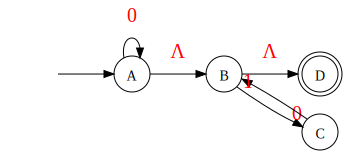
\includegraphics[scale=0.4]{images/2_seminar_lambdaelim}
\item Find $\delta^*(q,a)$ for alle $q\in Q$ og $a\in \Sigma$
\item Se om $\Lambda(\{q_0\})\cap A \neq \emptyset$
\begin{columns}
\column{5cm}
\scalebox{0.6}{
  \begin{tabular}{|c|ccc|cc|}
    \hline
    $q$ & $\delta(q,\Lambda)$ & $\delta(q, 0)$ & $\delta(q, 1)$ & $\delta^*(q,0)$ & $\delta^*(q,1)$\\
    \hline
    A & $\{B\}$ & $\{A\}$ & $\{\}$ & \{A,B,C,D\} & \{\} \\
    B & $\{D\}$ & $\{C\}$ & $\{\}$ & \{C,D\} & \{\} \\
    C & $\{\}$ & $\{\}$ & $\{B\}$ & \{\} & \{B,D\} \\
    D & $\{\}$ & $\{D\}$ & $\{\}$ & \{D\} & \{\} \\
    \hline
  \end{tabular}
  }
\column{5cm}
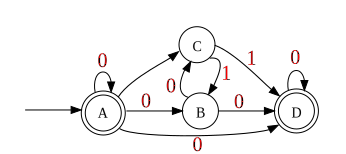
\includegraphics[scale=0.4]{images/2_seminar_lambdaelim2}
\end{columns}
\end{itemize}
\end{frame}
\begin{frame}
\frametitle{Bevis for korrekthed af $\Lambda $-eliminering}
\begin{itemize}[<+->]
\item Vi skal vise:  $\forall x\in \Sigma^*: x \in L(M1) \Leftrightarrow x\in L(M)$
  
$x=\Lambda$ :
brug definition af $A_1$ og $\Lambda$-lukning...
\item
$x\neq \Lambda$:
Lemma:  $\forall x\in \Sigma^*, x\neq \Lambda :  \delta *(q_0, x) = \delta_1*(q_0, x)$

...

\item
– se bogen Th. 4.2 p. 141.
\end{itemize}
\end{frame}
\begin{frame}
\frametitle{Øvelser}
\begin{itemize}
\item [Martin] Opg. 4.13 (p.159)
Kør strenge på en NFA-$\Lambda$
\item [Martin] Opg. 4.28 (e)
Brug algoritmen til $\Lambda$-eliminering
\end{itemize}
\end{frame}


\section{Kleenes sætning}
\subsection{Kleenes sætning del 1}
\begin{frame}
\frametitle{Status}
\begin{itemize}[<+->]
\item Vi har defineret 4 formalismer
regulære udtryk
FA,
NFA,
NFA-$\Lambda$
\item og er ved konstruktivt at bevise ækvivalens i udtrykskraft
\end{itemize}
\includegraphics[scale=0.4]{images/2_seminar_equiv}
\end{frame}

\begin{frame}
\frametitle{Ethvert regulært udtryk kan oversættes til en NFA-$\Lambda$}
(Kleenes sætning, del 1)
\begin{itemize}
\item Bevis:
  Induktion i strukturen af det regulære udtryk $r$.
\item
Vis konstruktivt for hvert tilfælde hvordan man kan lave den korrekte NFA-$\Lambda$
\end{itemize}
\end{frame}
\begin{frame}
\frametitle{Basis}
\begin{columns}
\column{5cm}
\begin{itemize}
\item 
$r=\emptyset$
\item $r=\Lambda$
\item $r=a,$ hvor $a\in\Sigma$
\end{itemize}
\column{5cm}
\begin{itemize}[<+->]
\item
\includegraphics[scale=0.4]{images/2_seminar_basis_emptyset}
\item
\includegraphics[scale=0.4]{images/2_seminar_basis_lambda}
\item
\includegraphics[scale=0.4]{images/2_seminar_basis_a}
\end{itemize}
\end{columns}
\end{frame}
\begin{frame}
\frametitle{Induktionsskridt}
\begin{itemize}[<+->]
\item For alle deludtryk $s$ af $r$ kan vi udnytte induktionshypotesen.
\item der eksisterer en NFA-$\Lambda$ $M_s$ hvor $L(M_s)=L(s)$
\item 
\begin{columns}
\column{5cm}$r=r_1+r_2$ \pause
\column{5cm}\includegraphics[scale=0.4]{images/2_seminar_kleene_1_add}
\end{columns}
\end{itemize}
\end{frame}
\begin{frame}
\frametitle{Induktionsskridt (part 2)}
\begin{columns}
\column{5cm}$r=r_1\cdot r_2$ \pause
\column{5cm}\includegraphics[scale=0.4]{images/2_seminar_kleene_1_times}
\end{columns} \pause
\begin{columns}
\column{5cm}$r=r_1^*$ \pause
\column{5cm}\includegraphics[scale=0.4]{images/2_seminar_kleene_1_star}
\end{columns}
\end{frame}

\begin{frame}
\frametitle{Formel beskrivelse og bevis for korrekthed}
Se beviset i bogen: p. 146
\end{frame}

\begin{frame}
\frametitle{Eksempel}
Konstruer en NFA-$\Lambda$ for det regulære udtryk $(00+1)^*(10)^*$
\begin{itemize}[<+->]
\item 0:
  \includegraphics[scale=0.4]{images/2_seminar_kleene_1_ex_0}
\item 1:
  \includegraphics[scale=0.4]{images/2_seminar_kleene_1_ex_1}
\item 00:
  \includegraphics[scale=0.4]{images/2_seminar_kleene_1_ex_00}
\item 10:
  \includegraphics[scale=0.4]{images/2_seminar_kleene_1_ex_10}
\end{itemize}
\end{frame}
\begin{frame}
\frametitle{Eksempel fortsat}
Konstruer en NFA-$\Lambda$ for det regulære udtryk $(00+1)^*(10)^*$
\begin{itemize}[<+->]
\item $00+1$:
  \includegraphics[scale=0.4]{images/2_seminar_kleene_1_ex_00plus1}
\item $(00+1)^*$:
  \includegraphics[scale=0.4]{images/2_seminar_kleene_1_ex_00plus1star}
\end{itemize}
\end{frame}
\begin{frame}
\frametitle{Eksempel fortsat}
Konstruer en NFA-$\Lambda$ for det regulære udtryk $(00+1)^*(10)^*$
\begin{itemize}[<+->]
\item $(10)^*$:
  \includegraphics[scale=0.4]{images/2_seminar_kleene_1_ex_10star}
\item $(00+1)^*(10)^*$:
  \includegraphics[scale=0.4]{images/2_seminar_kleene_1_ex_00plus1star10star}
\end{itemize}
\end{frame}
\begin{frame}
\frametitle{Øvelser}
\begin{itemize}
\item [Martin] Opg. 4.35 (a) (p. 163)\\
Udfør algoritmen for konstruktion af NFA-$\Lambda$ fra regulært udtryk. 
\end{itemize}
\end{frame}
\subsection{Kleenes sætning del 2}
\begin{frame}
  \frametitle{Enhver FA kan oversættes til et regulært udtryk}
Kleene's sætning del 2.

Vi laver bevis med induktion naturligvis, men induktion i hvad?
\end{frame}

\begin{frame}
\frametitle{Fra FA til regulært udtryk}
\begin{itemize}[<+->]
\item For en FA $M=(Q, \Sigma , q_0, A, \delta )$ er $L(M)$ defineret som
	$L(M) = \{ x\in \Sigma^* | \delta^*(q_0, x)\in A \}$
\item Da A er endelig kan L(M) udtrykkes som en endelig forening af sprog på form
	 $L(p, q) = \{ x\in \Sigma^* | \delta^*(p, x)=q \}$
\item Vi vil vise at hvert af disse sprog kan oversættes til et regulært udtryk, $r(p, q)$, og derefter kombinere disse med “+”
\end{itemize}
\end{frame}
\begin{frame}
\frametitle{Induktion i antal tilstande}
\begin{itemize}[<+->]
\item Antag tilstandene i M er nummereret $1, ..., |Q|$
\item Definer $L(p, q, k)$ hvor $p,q\in Q$ og $k\in \{1..|Q|\}$ som
  mængden af strenge, der fører fra p til q og kun går gennem
  tilstande med nummer $\leq k$ (fraregnet endepunkterne)
  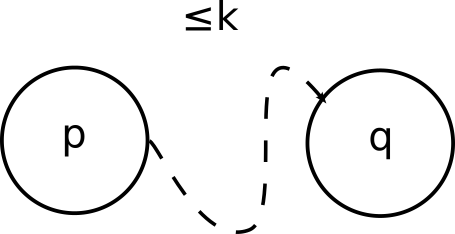
\includegraphics[scale=0.2]{images/2_seminar_kleene_2_lessk}
\item dvs.  $L(p, q) = L(p, q, |Q|)$
\item Vi vil vise ved induktion i $k$ at $L(p, q, k)$ svarer til 
et regulært udtryk, $r(p, q, k)$
\item dvs. vælg  $r(p, q) = r(p, q, |Q|)$
\end{itemize}
\end{frame}
\begin{frame}
\frametitle{Basis}
$k = 0$
\begin{itemize}[<+->]
\item 
$L(p, q, 0)$ er mængden af strenge, der fører fra 
$p$ til $q$ uden at gå gennem nogen tilstande 
(fraregnet endepunkterne)
\item
hvis $p\neq q$: 
$L(p, q, 0) = \{ a\in \Sigma  | \delta (p, a) = q \}$
\item
hvis $p=q$: 
$L(p, q, 0) = \{ a\in \Sigma  | \delta (p, a) = p \} \cup \{\Lambda\}$
\item
dvs. vi kan altid finde et regulært udtryk 
$r(p, q, 0)$ for $L(p, q, 0)$
\end{itemize}
\end{frame}
\begin{frame}
\frametitle{Induktionsskridt}
$k+1$
\begin{itemize}[<+->]
\item $L(p, q, k + 1)$ er mængden af strenge, der fører fra $p$ til $q$ 
og kun går gennem tilstande med nummer $\leq k + 1$
\item
To tilfælde:

\begin{itemize}[<+->]
\item 
  Strenge der ikke går gennem tilstand $k + 1$: $L(p, q, k)$ 
\item Strenge
  der går gennem tilstand $k + 1$: $L(p, k + 1, k) L(k + 1, k + 1, k)^*
  L(k + 1, q, k)$
\end{itemize}
\item dvs. $L(p, q, k + 1) = L(p, q, k) \cup 
			    L(p, k + 1, k) L(k + 1, k + 1, k)^* L(k + 1, q, k)$
\item som vha. induktionshypotesen svarer til et regulært udtryk 
	$r(p, q, k + 1) = r(p, q, k) + 
			    r(p, k + 1, k) r(k + 1, k + 1, k)^* r(k + 1, q, k)$
\end{itemize}
\end{frame}
\begin{frame}
\frametitle{Eksempel}
Oversæt denne FA til et regulært udtryk
\includegraphics[scale=0.4]{images/2_seminar_kleene_2_ex.png}
\begin{itemize}[<+->]
\item $r = r(1,1,3) + r(1,2,3)$
\item $r(1,1,3) = r(1,1,2) + r(1,3,2)r(3,3,2)^*r(3,1,2)$
\item $r(1,1,2) = r(1,1,1) + r(1,2,1)r(2,2,1)^*r(2,1,1)$
\item $r(1,1,1) = r(1,1,0) + r(1,1,0)r(1,1,0)^*r(1,1,0)$
\item $r(1,1,0) = a + \Lambda$
\item Heldigvis kan vi sætte en computer til det!
\end{itemize}
\end{frame}
\begin{frame}
\frametitle{Eksempel fortsat}
\begin{itemize}[<+->]
\item \tiny{$r = ((\emptyset+(((((\emptyset +a)+\lambda)+(\emptyset (((\emptyset +\lambda )^*)$$(\emptyset +a))))+((((\emptyset +a)+\lambda )+(\emptyset (((\emptyset +\lambda )^*)(\emptyset +a) )))$$(((((\emptyset +a)+\lambda )+(\emptyset (((\emptyset +\lambda )^*)(\emptyset +a))))^*)(((\emptyset +a)+\lambda )+(\emptyset (((\emptyset +\lambda )^*)(\emptyset +a)))))))+((((\emptyset +b)+(\emptyset (((\emptyset +\lambda )^*)(\emptyset +b))))+((((\emptyset +a)+\lambda )+(\emptyset (((\emptyset +\lambda )^*)(\emptyset +a))))(((((\emptyset +a)+\lambda )+(\emptyset (((\emptyset +\lambda )^*)(\emptyset +a))))^*)((\emptyset +b)+(\emptyset (((\emptyset +\lambda )^*)(\emptyset +b)))))))(((((\emptyset +\lambda )+((\emptyset +b)(((\emptyset +\lambda )^*)(\emptyset +b))))+(((\emptyset +a)+((\emptyset +b)(((\emptyset +\lambda )^*)(\emptyset +a))))(((((\emptyset +a)+\lambda )+(\emptyset (((\emptyset +\lambda )^*)(\emptyset +a))))^*)((\emptyset +b)+(\emptyset (((\emptyset +\lambda )^*)(\emptyset +b)))))))^*)(((\emptyset +a)+((\emptyset +b)(((\emptyset +\lambda )^*)(\emptyset +a))))+(((\emptyset +a)+((\emptyset +b)(((\emptyset +\lambda )^*)(\emptyset +a))))(((((\emptyset +a)+\lambda )+(\emptyset (((\emptyset +\lambda )^*)(\emptyset +a))))^*)(((\emptyset +a)+\lambda )+(\emptyset (((\emptyset +\lambda )^*)(\emptyset +a)))))))))))+((((\emptyset +b)+(\emptyset (((\emptyset +\lambda )^*)(\emptyset +b))))+((((\emptyset +a)+\lambda )+(\emptyset (((\emptyset +\lambda )^*)(\emptyset +a))))(((((\emptyset +a)+\lambda )+(\emptyset (((\emptyset +\lambda )^*)(\emptyset +a))))^*)((\emptyset +b)+(\emptyset (((\emptyset +\lambda )^*)(\emptyset +b)))))))+((((\emptyset +b)+(\emptyset (((\emptyset +\lambda )^*)(\emptyset +b))))+((((\emptyset +a)+\lambda )+(\emptyset (((\emptyset +\lambda )^*)(\emptyset +a))))(((((\emptyset +a)+\lambda )+(\emptyset (((\emptyset +\lambda )^*)(\emptyset +a))))^*)((\emptyset +b)+(\emptyset (((\emptyset +\lambda )^*)(\emptyset +b)))))))(((((\emptyset +\lambda )+((\emptyset +b)(((\emptyset +\lambda )^*)(\emptyset +b))))+(((\emptyset +a)+((\emptyset +b)(((\emptyset +\lambda )^*)(\emptyset +a))))(((((\emptyset +a)+\lambda )+(\emptyset (((\emptyset +\lambda )^*)(\emptyset +a))))^*)((\emptyset +b)+(\emptyset (((\emptyset +\lambda )^*)(\emptyset +b)))))))^*)(((\emptyset +\lambda )+((\emptyset +b)(((\emptyset +\lambda )^*)(\emptyset +b))))+(((\emptyset +a)+((\emptyset +b)(((\emptyset +\lambda )^*)(\emptyset +a))))(((((\emptyset +a)+\lambda )+(\emptyset (((\emptyset +\lambda )^*)(\emptyset +a))))^*)((\emptyset +b)+(\emptyset (((\emptyset +\lambda )^*)(\emptyset +b))))))))))) $}
\item (Hvis programmet ikke simplificerer undervejs...)
\end{itemize}
\end{frame}
\begin{frame}
\frametitle{Øvelser}
\begin{itemize}
\item [Martin] Opg. 4.38(b) (p. 164)\\
Brug algoritmen fra Kleenes sætning del 2.
\end{itemize}
\end{frame}

\section{Frokost}
\begin{frame}
  \begin{center}
    \includegraphics{images/lunch}
  \end{center}
\end{frame}
\begin{frame}
\frametitle{Resume}
\begin{itemize}
\item Regulære udtryk, FA’er, NFA’er og NFA-$\Lambda$’er
svarer alle til klassen af regulære sprog
\item Algoritmer fra de konstruktive beviser:
\item determinisering (delmængdekonstruktionen)
\item $\Lambda$-eliminering
\item regulært udtryk $\rightarrow$  NFA-$\Lambda$
\item FA $\rightarrow$ regulære udtryk (primært et teoretisk resultat)
\end{itemize}
\end{frame}
\section{Minimering}
\subsection{MyHill Nerode}
\begin{frame}
\frametitle{Karakteristik af de regulære sprog}
Et sprog er regulært hviss (hvis og kun hvis)
\begin{itemize}[<+->]
\item L beskrives af et regulært udtryk
\item L genkendes af en FA/NFA/NFA-$\Lambda$
\item \alert{Der ikke findes uendeligt mange strenge der er parvist
  skelnelige mht. L}
\end{itemize}
\end{frame}

\begin{frame}
\frametitle{Skelnelighed (fra 1. seminar)}
\begin{itemize}[<+->]
\item x og y er skelnelige mht. L hvis
$\exists z\in \Sigma^*: (xz\in L \wedge  yz\not\in L) \vee 
	      (xz\not\in L \wedge  yz\in L)$
\item
  Hvis to skelnelige strenge mht. L køres på en FA, 
  der accepterer L, vil de ende i forskellige tilstande
\item
Intuition bag FA-minimering:  
\item hvis to strenge er \alert{uskelnelige} mht. FA’ens sprog, er der ingen grund til at den skelner mellem dem!
\end{itemize}
\end{frame}

\begin{frame}
\frametitle{Uskelnelighedsrelationen $I_L$}
\begin{itemize}[<+->]
\item Definition:       
Givet et sprog $L\subseteq \Sigma^*$, definer 
relationen $I_L$ over $\Sigma^*$ ved:
		$x I_L y   \Leftrightarrow$   $x$ og $y$ er uskelnelige mht. $L$
\end{itemize}
\end{frame}

\begin{frame}
\frametitle{Relationer}
\begin{itemize}[<+->]
\item En (binær) relation $R$ over en mængde $A$ er 
en delmængde af $A\times A$
\item
Eksempler:
 $\leq$  er en relation over mængden af reelle tal
 $I_L$ er en relation over $\Sigma^*$
\item
Notation:    $x R y   \Leftrightarrow   (x,y)\in R$
\end{itemize}
\end{frame}

\begin{frame}
\frametitle{Ækvivalensrelationer}
\begin{itemize}[<+->]
\item R er en ækvivalensrelation hvis den er
  \item
refleksiv  $(\forall x:  x R x)$
\item
symmetrisk $(\forall x,y:  x R y \Rightarrow y R x)$
\item
transitiv $(\forall x,y,z:  x R y \wedge  y R z \Rightarrow x R z)$
\item
En ækvivalensrelation over A definerer 
en partitionering af A
\includegraphics[scale=0.4]{images/2_seminar_equivclasses}
\item
Notation:  $[x] = \{y | x R y\}$ kaldes 
ækvivalensklassen for x mht. R
\end{itemize}
\end{frame}

\begin{frame}
\frametitle{Egenskaber ved $I_L$}
\begin{itemize}[<+->]
\item $I_L$ er
\item refleksiv  $(\forall x:  x I_L x)$
\item symmetrisk $(\forall x,y:  x I_L y \Rightarrow  y I_L x)$
\item transitiv $(\forall x,y,z:  x I_L y \wedge  y I_L z \Rightarrow  x I_L z)$
\item dvs. $I_L$ er en ækvivalensrelation
\item
$I_L$ partitionerer $\Sigma^*$
\item
$[x]$ er mængden af strenge, der er uskelnelige fra $x$ mht. $L$
\end{itemize}
\end{frame}

\begin{frame}
\frametitle{Quiz}
$L = \{0,1\}^*\{10\}$ \\
Beskriv ækvivalensklasserne for $I_L$
\begin{itemize}
\item \visible<2->{Hint:  der er 3 ækvivalensklasser...}
\includegraphics[scale=0.4]{images/2_seminar_equivclassessigma}
\item \visible<3->{Hint:  find en streng, der er skelnelig fra $\Lambda$ ...}
\item \visible<4->{Hint:  find en streng, der er skelnelig 
  fra både $\Lambda$ og 1...}
\end{itemize}
\visible<5->{
\[X:  \{\Lambda , 0\} \cup \{0,1\}^*\{00\} = [\Lambda ]\]
\[Y:  \{0,1\}^*\{1\} = [1]\]
\[Z:  \{0,1\}^*\{10\} = [10]\]
}
\end{frame}

\begin{frame}
\frametitle{MyHill-Nerode-sætningen}
\begin{itemize}[<+->]
\item $L$ er regulært $\Leftrightarrow I_L$ har endeligt mange 				      ækvivalensklasser
\item “$\Rightarrow$”: (1. seminar) hvis $I_L$ har uendeligt mange 
	 ækvivalensklasser, så er $L$ ikke regulært
\item “$\Leftarrow$”: Bevis følger...
\end{itemize}
\end{frame}

\begin{frame}
\frametitle{Konstruktion af en FA fra $I_L$}
\begin{itemize}[<+->]
\item Givet et sprog $L\subseteq \Sigma^*$, antag $I_L$ har 
endeligt mange ækvivalensklasser.
\item
Vi kan definere en FA, hvor tilstandene er ækvivalensklasserne af $I_L$
\end{itemize}
\end{frame}

\begin{frame}
\frametitle{Eksempel}
\begin{itemize}
\item Ækvivalensklasserne for $I_L$ når $L = \{0,1\}^*\{10\}$ :
\[X:  \{\Lambda , 0\} \cup \{0,1\}^*\{00\} = [\Lambda ]\]
\[Y:  \{0,1\}^*\{1\} = [1]\]
\[Z:  \{0,1\}^*\{10\} = [10]\]
\begin{columns}
\column{5cm}
\includegraphics[scale=0.4]{images/2_seminar_equivclassessigma}
\column{5cm}
$M_L$:\includegraphics[scale=0.4]{images/2_seminar_myhillfa}
\end{columns}
\end{itemize}
\end{frame}

\begin{frame}
\frametitle{Konstruktion af en FA fra $I_L$}
\begin{itemize}[<+->]
\item Definer en FA: 
	$M_L=(Q, \Sigma , q_0, A, \delta)$ hvor
\item $Q = Q_L$    hvor $Q_L$ er ækvivalensklasserne af $I_L$
\item $q_0 = [\Lambda ]$
\item $A = \{ q\in Q | q \cap L \neq  \emptyset \}$
\item $\delta (q, a) = p$   hvis $q=[x]$ og $p=[xa]$ for en streng x
	($\delta$  er veldefineret idet  $x I_L y \Rightarrow  xa I_L ya$)
\item
Påstand: $L(M_L) = L$
\end{itemize}
\end{frame}

\begin{frame}
\frametitle{Quiz}
\begin{itemize}
\item Antag ækvivalensklasserne for $I_L$ er 
\[X = \{x\in \{0,1\}^* | \text{antal 1’er i } x \text{ er lige } \}\]
\[Y = \{x\in \{0,1\}^* | \text{antal 1’er i } x \text{ er ulige } \}\]
og $111\in L$

Lav en FA, der accepterer L
\end{itemize}
\begin{columns}
\column{5cm}
\visible<2->{\includegraphics[scale=0.4]{images/2_seminar_equivclassesodd}}
\column{5cm}
\visible<3->{\includegraphics[scale=0.4]{images/2_seminar_odd1}}
\end{columns}
\end{frame}

\begin{frame}
\frametitle{Bevis for korrekthed af konstruktionen}
\begin{itemize}[<+->]
\item Påstand: $L(M_L) = L$
\item Lemma:  $\forall x,y\in \Sigma^*:   \delta^*([x], y) = [xy]$
\item Bevis: induktion i strukturen af $y$...
\item $\delta^*(q_0, x) = \delta^*([\Lambda ], x) = [x]$  (følger af lemmaet og def. af $q_0$)
\item $x\in L(M_L)\Leftrightarrow\delta^*(q_0, x)\in A\Leftrightarrow [x]\in A\Leftrightarrow [x] \cap L 
\neq \emptyset$
\item $x\in L  \Rightarrow   [x] \cap  L \neq  \emptyset $   (da $x\in [x]$)
\item $[x] \cap  L \neq  \emptyset  \Rightarrow   x\in L$    (bruger def. af $I_L$)
\item dvs.  $x\in L(M_L)  \Leftrightarrow  x\in L$
\end{itemize}
\end{frame}

\begin{frame}
  \frametitle{Øvelser}
\begin{itemize}
\item{} [Martin] Opg. 5.2 (p. 191)
  Find selv ækvivalensklasser
\item{} [Martin] Opg. 5.7
  Konstruer en FA ud fra en beskrivelse af $I_L$
\end{itemize}
\end{frame}

\begin{frame}
\frametitle{Minimering af automater}
\begin{center}
\includegraphics[scale=0.4]{images/2_seminar_minimize}
\end{center}
\begin{itemize}
\item Man kan i visse tilfælde opnå en mindre FA 
ved at “slå tilstande sammen”...
\item Kan vi gøre det systematisk?
\item Vil den resulterende FA blive minimal?
\end{itemize}
\end{frame}

\begin{frame}
\frametitle{En algoritme til FA-minimering}
Fra MyHill-Nerode-sætningen kan vi udlede
en algoritme, der 
givet en vilkårlig FA $M=(Q, \Sigma , q_0, A, \delta)$, 
finder en minimal FA $M_1$ hvor $L(M_1)=L(M)$
\end{frame}

\begin{frame}
\frametitle{To partitioneringer af $\Sigma^*$}
\begin{itemize}[<+->]
\item 1:	Ækvivalensklasserne af $I_L$
(svarer til tilstandene i den minimale FA $M_L$)
\item 2:	En opdeling af alle $x\in \Sigma^*$ efter værdien af $\delta^*(q_0, x)$
(svarer til tilstandene i den givne FA M)	
\item Kan vi konstruere 1 ud fra 2?
\item Definer for alle $q\in Q$:
	$L_q = \{ x\in \Sigma^* | \delta^*(q_0, x) = q \}$
\end{itemize}
\end{frame}


\begin{frame}
  \frametitle{Eksempel}
\includegraphics[scale=0.4]{images/2_seminar_minimize}\\
\includegraphics[scale=0.4]{images/2_seminar_minimizeequiv}
\end{frame}

\begin{frame}
\frametitle{Fjern uopnåelige tilstande}
\begin{itemize}[<+->]
\item Ækvivalensklasserne af $I_L$ indeholder alle 
mindst 1 streng
\item Det er muligt at $L_q = \emptyset$ for en eller flere $q\in Q$
(hvis $q$ er uopnåelig fra $q_0$)
\item
Der findes en algoritme, der kan fjerne uopnåelige tilstande fra en FA uden at ændre sproget
\item
Vi kan derfor antage at $Lq \neq  \emptyset$ for alle $q\in Q$
\end{itemize}
\end{frame}

\begin{frame}
\frametitle{Opnåelige tilstande}
\begin{itemize}[<+->]
\item Givet en  FA $M=(Q, \Sigma , q_0, A, \delta)$
\item Lad R være den mindste mængde, der opfylder:
\item $q_0\in R$
\item $\forall q\in R, a\in \Sigma :  \delta (q, a)\in R$
\item $R$ er mængden af opnåelige tilstande i $M$
\item (minder om def. af $\Lambda-lukning$)
\end{itemize}
\end{frame}

\begin{frame}
\frametitle{Fixpunktsalgoritme}
\begin{itemize}[<+->]
\item R kan findes med en fixpunktsalgoritme:
\begin{center}
  \includegraphics[scale=0.4]{images/2_seminar_fixpoint}
\end{center}
\item $1\in R$
\item $\delta (1, b)=2\in R$
\item $\delta (2, a)=4\in R$
\item fixpunkt er nu nået\\
dvs. de opnåelige tilstande er $R=\{1,2,4\}$
\end{itemize}
\end{frame}

\begin{frame}
\frametitle{Forholdet mellem partition 1 og 2}
\begin{itemize}[<+->]
\item Fra seminar 1: $\delta^*(q_0, x)=\delta^*(q_0, y)  \Rightarrow  x I_L y$
\item Dvs. enhver $L_q$–mængde er helt indeholdt i 
én $I_L$-ækvivalensklasse
\item
Enhver ækvivalensklasse af $I_L$ er derfor foreningen af 
en eller flere af $L_q$–mængderne
\item
Da $L_q \neq \emptyset$ er hver af disse foreninger unik
\item
Definition: $p \equiv q  \Leftrightarrow  L_p \text{ og } L_q$ er delmængder
af samme $I_L$-ækvivalensklasse
\item
Dvs. hvis $p \equiv q$, så svarer $p$ og $q$ til samme tilstand i den minimale automat!
\end{itemize}
\end{frame}

\begin{frame}
\frametitle{Konstruktion af $\equiv$  (minimeringsalgoritmen)}
\begin{itemize}[<+->]
\item Lad S være den mindste mængde, der opfylder: 
\item a) $(p\in A \wedge  q\not\in A) \vee  (p\not\in A \wedge  q\in A) \Rightarrow (p, q)\in S$
\item b) $(\exists a\in \Sigma : (\delta (p, a), \delta (q, a))\in S)   \Rightarrow    (p, q)\in S$
\item
Påstand:  $p \equiv q$ hvis og kun hvis $(p, q)\in S$

S kan beregnes med en fixpunktsalgoritme 
(i stil med opnåelige tilstande og $\Lambda$-lukning tidligere...)
\end{itemize}
\end{frame}

\begin{frame}
\frametitle{Eksempel}
\begin{columns}
\column{4cm}\only<-8>{\includegraphics[scale=0.35]{images/2_seminar_min_ex_1}}
\only<9->{\includegraphics[scale=0.35]{images/2_seminar_min_ex_2}}
\column{2.5cm}
\visible<10->{\includegraphics[scale=0.35]{images/2_seminar_min_ex_3}}
\column{3.5cm}
\scalebox{.5}{
\begin{tabular}{c|c|c|c|c|c|c|}
  2 &  \\
  3 & \visible<7->{X} & \visible<7->{X}  \\
  4 &   &   & \visible<7->{X} \\
  5 & \visible<7->{X} & \visible<7->{X} &   & \visible<7->{X} \\
  6 & \visible<4->{\visible<4->{X}} & \visible<4->{\visible<4->{X}} & \visible<4->{X} & \visible<4->{X} & \visible<4->{X} \\
  7 & \visible<7->{X} & \visible<7->{X} &   & \visible<7->{X} &   & \visible<7->{X}  \\
  \hline
    & 1 & 2 & 3 & 4 & 5 & 6
\end{tabular}
}
\end{columns}
\begin{itemize}
\item<1-> Find alle par af tilstande
\item<2-> Fjern uopnåelige tilstande (ingen i denne FA)
\item<3-> Marker alle par som med/ikke med i $A$
\item<6-> Find $\equiv$  ved at udfylde en tabel for $S$ (fixpunktsberegning)
\item<8-> Kombiner tilstande, der svarer til umærkede par
\end{itemize}
\end{frame}


\begin{frame}
\frametitle{Bevis for korrekthed af minimeringsalgoritmen}
\begin{itemize}[<+->]
\item Antag $p,q\in Q, x\in L_p, y\in L_q$\\
(dvs. $\delta^*(q_0, x)=p$ og $\delta^*(q_0, y)=q$)
\item
Lemma:  Følgende udsagn er ækvivalente:
\[p \equiv q\]
\[x I_L y\]
\[\forall z\in \Sigma^*:  \delta^*(p, z)\in A  \Leftrightarrow	\delta^*(q, z)\in A\]
\end{itemize}
\end{frame}

\begin{frame}
\frametitle{Bevis for korrekthed, fortsat}
\begin{itemize}[<+->]
\item Påstand:  $p \equiv q$ hvis og kun hvis $(p, q)\not\in S$
\item
Iflg. lemmaet:
\begin{align*}
p \not\equiv q \Leftrightarrow (\exists z\in \Sigma^*:  (&\delta^*(p, z)\in A \wedge \delta^*(q, z)\not\in A) \vee \\
 & (\delta^*(p, z)\not\in A \wedge  \delta^*(q, z)\in A))
\end{align*}
\item
$p \not\equiv q \Rightarrow (p, q)\in S$    (brug lemmaet, lav induktion i $z$)
\item
$(p, q)\in S \Rightarrow p \not\equiv q$     (brug lemmaet, lav induktion i $S$)
\end{itemize}
\end{frame}

\begin{frame}
\frametitle{Øvelse}
\begin{itemize}
\item{} [Martin] 5.16 (a+e) (p.192)
\end{itemize}
\end{frame}

\section{Java projekt}
\begin{frame}
\frametitle{Regaut pakken}
\begin{itemize}[<+->]
\item Udleverede programdele:
\item \texttt{NFA.java} og \texttt{NFALambda.java}:
	repræsentation af NFA’er og NFA-$\Lambda$’er
\item \texttt{RegExp.java}:
	repræsentation af regulære udtryk
\item parser for regulære udtryk
\item de trivielle oversættelser: $FA \rightarrow  NFA, NFA \rightarrow  NFA-\Lambda$
\end{itemize}
\end{frame}
\begin{frame}
\frametitle{NFA.java}
\begin{itemize}[<+->]
\item Repræsentation som \texttt{FA.java}, med én undtagelse:
	
\item \texttt{transitions} er en funktion fra \texttt{StateSymbolPair}
  til en \alert{mængde} af \texttt{State} objekter
\end{itemize}
\end{frame}
\begin{frame}
\frametitle{NFALambda.java}
\begin{itemize}[<+->]
\item Repræsentation som NFA.java, med én undtagelse:
\item $\Lambda$ repræsenteres som \texttt{$\backslash$uFFFF}  (= \texttt{NFALambda.LAMBDA})
\end{itemize}
\end{frame}

\begin{frame}
\frametitle{RegExp.java}
\begin{itemize}[<+->]
\item \texttt{RegExp(String, Alphabet)}
 – parser et regulært udtryk
\item
\texttt{toString()}
 – til udskrift af et parsed regulært udtryk
\item
\texttt{toNFALambda()}
 – konstruktionen fra Kleene’s sætning del 1
\item
\texttt{simplify()}
 – simplificerer et parsed regulært udtryk, 
nyttig efter FA.toRegExp() (Kleene’s sætning del 2)
\end{itemize}
\end{frame}

\begin{frame}
\frametitle{Minimering i dRegAut java-pakken}
\begin{itemize}[<+->]
\item ”pseudo-kode”:\\
  uformel mellemting mellem 
  de matematiske definitioner 
og Java-koden
\end{itemize}
\end{frame}

\begin{frame}
\frametitle{FA.minimize()}
FA minimize() \{\\
\ \ phase 1: Remove unreachable states\\
\ \ phase 2a: Divide into accept/reject states\\
\ \ phase 2b: Iteration\\
\ \ phase 3: Build and return resulting minimal automaton n\\
\}
\end{frame}

\begin{frame}
\frametitle{FA.findReachableStates(), version 1}
Set findReachableStates() $\{$\\
\ \ $R = \{ q_0 \}$\\
\ \ $done = false$\\
\ \ while not done do\\
\ \ \ \ done = true\\
\ \ \ \ for each $q\in R$ do\\
\ \ \ \ \ \ for each $a\in \Sigma$ do\\
\ \ \ \ \ \ \ \ $p = \delta (q, a)$\\
\ \ \ \ \ \ \ \ if $p\not\in R$ then \\
\ \ \ \ \ \ \ \ \ \ add $p$ to $R$\\
\ \ \ \ \ \ \ \ \ \ $done = false$\\
\ \ return R\\
$\}$
\end{frame}

\begin{frame}
\frametitle{FA.findReachableStates(), version 2}

Vi kan holde øje med hvilke tilstande der ikke er ``færdigbesøgt'' for
at undgå at besøge hver tilstand flere gange:\\[.3cm]
Set findReachableStates() $\{$\\
\ \ $R = \{ \}$\\
\ \ $pending = \{ q_0 \}$\\
\ \ while $pending\neq \emptyset$ do\\
\ \ \ \ pick and remove an element $q$ from $pending$\\
\ \ \ \ add $q$ to $R$\\
\ \ \ \ for each $c\in \Sigma$  do\\
\ \ \ \ \ \ $p = \delta(q, c)$\\
\ \ \ \ \ \ if $p\not\in R$ then add $p$ to $pending$\\
\ \ return R\\
$\}$\\
\end{frame}

\begin{frame}
\frametitle{FA.minimize phase 2a}
\begin{itemize}
\item Define some ordering on the states $Q$
\item Declare marks: a set of pairs $(p,q)$ where $p,q\in Q$ and $p<q$
\item $marks=\emptyset$
\item for each pair $p,q\in Q$ where $p<q$ do\\
  \ \ if not $(p\in A \Leftrightarrow q\in A)$ then\\
  \ \ \ \ add $(p,q)$ to marks
\end{itemize}
Mange muligheder for Java-representation af marks...
\end{frame}

\begin{frame}
\frametitle{FA.minimize() phase 2b}
$done = false$\\
while not done do\\
\ \ done = true\\
\ \ for each pair $p,q\in Q$ where $p<q$ do\\
\ \ \ \  if $(p,q)\not\in$ marks then\\
\ \ \ \ \ \ for each $a\in \Sigma$  do\\
\ \ \ \ \ \ \ \ $r = \delta (p, a)$\\
\ \ \ \ \ \ \ \ $s = \delta (q, a)$\\
\ \ \ \ \ \ \ \ if $r >s$ then swap $r$ and $s$\\
\ \ \ \ \ \ \ \ if $(r,s)\in marks$ then\\
\ \ \ \ \ \ \ \ \ \ add $(p,q)$ to marks\\
\ \ \ \ \ \ \ \ \ \ $done = false$
\\ Kunne gøres smartere med en pending worklist.
\end{frame}

\begin{frame}
\frametitle{FA.minimize(), phase 3}
\small{
FA n = new FA with same alphabet as f
       but with no states or transitions yet\\
initialize empty maps old2new: $f.Q \rightarrow  n.Q$  and new2old: $n.Q \rightarrow  f.Q$\\
for each $r\in f.Q$ in order do\\
\ \ if $(s,r)\in marks$ for every $s<r$ then\\
\ \ \ \ add a new state p to $n.Q$\\
\ \ \ \ add $old2new(r) = p$ and $new2old(p) = r$\\
\ \ \ \ if $r\in f.A$ then add p to $n.A$\\
\ \ else\\
\ \ \ \ add $old2new(r) = old2new(s)$\\
\ \ if $r = f.q_0$  then set $n.q_0 = old2new(r)$\\
\ \ for each state $p \in n$ do\\
\ \ \ \ add $n.\delta(p,c) = old2new(f.\delta (new2old(p),c))$  for each $c\in \Sigma$ 
}
\end{frame}

\begin{frame}[fragile]

\frametitle{Eksempel}
\begin{verbatim}
Alphabet a = new Alphabet(‘0’, ‘1’);
RegExp r = new RegExp(“0+(1*+01*+10*+001*01)*0*”, a);

NFALambda n1 = r.toNFALambda();
NFA n2 = n1.removeLambdas();
FA n3 = n2.determinize();

System.out.println(“Før: ”+n3.getNumberOfStates());
FA n4 = n3.minimize();
System.out.println(“Efter: ”+n4.getNumberOfStates());
\end{verbatim}
\pause
Før: 13\\
\pause
Efter: 1
\end{frame}
\begin{frame}
\frametitle{Resume}
\begin{itemize}
\item MyHill-Nerode-sætningen: 
\item endnu en karakteristik af de regulære sprog
\item en algoritme til FA minimering
\item en algoritme til at fjerne uopnåelige tilstande i en FA
\end{itemize}
\end{frame}
\end{document}




%%% Local Variables: 
%%% mode: latex
%%% TeX-master: t
%%% End: 
